\documentclass[a4paper]{article}
\usepackage{amsmath,amssymb,amsthm}

% for flow chart
\usepackage{tikz}
\usetikzlibrary{shapes,arrows}
\tikzstyle{block} = [rectangle, draw, 
    text width=7em, text centered, rounded corners, minimum height=4em]
\tikzstyle{arrow} = [thick,->,>=stealth]

% for the laplace operator
\DeclareMathOperator{\Lapl}{\mathcal{L}}

% Set up remark environment with amsthm
\theoremstyle{remark}
\newtheorem*{remark}{Remark}
\newtheorem*{solution}{Solution}
\theoremstyle{theorem}
\newtheorem{theorem}{Theorem}
\newtheorem{example}{Example}

\title{The Laplace Transform}
\author{Darren Wee\\\texttt{darren.wee@u.nus.edu}}

\begin{document}
\maketitle

\section{The Basic Idea}
\begin{figure}[hbtp]
	\centering
	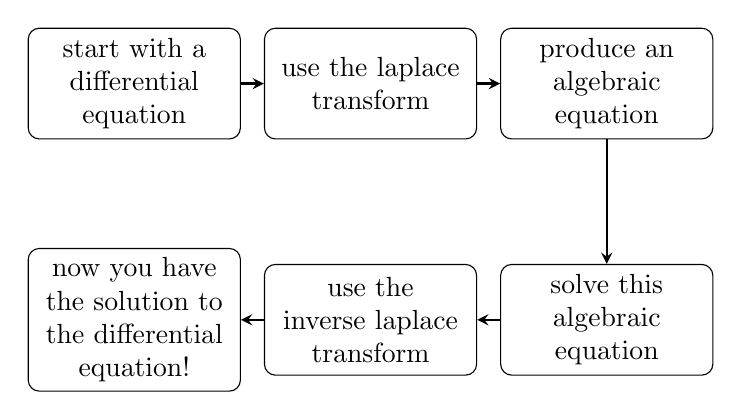
\begin{tikzpicture}[scale=1, node distance = 3cm, auto]
		% draw the text boxes first
		\node [block] (start) {start with a differential equation};
		\node [block, right of=start] (usetransform) {use the laplace transform};
		\node [block, right of=usetransform] (produce) {produce an algebraic equation};
		\node [block, below of=produce] (solve) {solve this algebraic equation};
		\node [block, left of=solve] (useinverse) {use the inverse laplace transform};
		\node [block, left of=useinverse] (solution) {now you have the solution to the differential equation!};
	
		% draw the edges connecting text boxes
		\draw [arrow] (start) -- (usetransform);
		\draw [arrow] (usetransform) -- (produce);
		\draw [arrow] (produce) -- (solve);
		\draw [arrow] (solve) -- (useinverse);
		\draw [arrow] (useinverse) -- (solution);
	\end{tikzpicture}
\end{figure}

\section{The Laplace Transform}
\subsection{Definition}
Suppose $f(t)$ is a function of $t$.
The Laplace transform of $f$ is the following function of $s$ where $s>0$ is given by
\begin{equation}
	\Lapl{(f)(s)} = F(s) = \int_0^\infty f(t)e^{-st}\: dt
\end{equation}

\begin{theorem}
	For any function $h$ defined on $[0, \infty)$,
	\begin{equation}
		\int_0^\infty h(t)\:dt = \lim_{w\to\infty} \int_0^w h(t)\:dt
	\end{equation}

	The integral is said to \emph{converge} if this limit exists.
\end{theorem}

\begin{example}
	Complete the Laplace transform of $f(t) = t$.
\end{example}

\begin{solution}
	\begin{equation}
		F(s) = \int_0^\infty te^{-st}\:dt
	\end{equation}
	
	Here, we must integrate by parts\footnote{$\int u(x)v'(x)\:dx = u(x)v(x) - \int u'(x)v(x)\:dx$}

	Suppose we solve the \emph{indefinite} integral first.	
	\begin{align}
		F(s) 	= & \int te^{-st}\:dt \\
				= & t\Big(\frac{e^{-st}}{-s}\Big) - \int \frac{e^{-st}}{-s}\:dt \\
				= & t\Big(\frac{e^{-st}}{-s}\Big) - \frac{1}{s^2}e^{-st} + C
	\end{align}

	Now to solve for the \emph{definite} integral, we take the limit
	\begin{align}
		\lim_{w\to\infty} \Big[ t\Big(\frac{e^{-st}}{-s}\Big) - \frac{1}{s^2}e^{-st}\Big] \Big|_{t=0}^{t=w}\\
		& = \lim_{w\to\infty} \Big[ w\Big(\frac{e^{-sw}}{-s}\Big) -\frac{1}{s^2}(e^{-sw}) - \Big(0-\frac{1}{s^2}\Big) \Big] \\
		& = \lim_{w\to\infty} \Big[ -\frac{1}{s}(we^{-sw}) - \frac{1}{s^2}e^{-sw} + \frac{1}{s^2} \Big]\\
		\text{Applying L'Hopital's Rule,}\\
		& = \lim_{w\to\infty} \Big[\frac{1}{s^2}\Big] \\
		& = \frac{1}{s^2} 
	\end{align}

	Therefore we see that $F(s) = \frac{1}{s^2}$.
\end{solution}

\subsection{Some Useful Identities}
\begin{equation}
	\Lapl{(e^{at})} = \frac{1}{s-a} \text{ for } s > a
\end{equation}
\begin{equation}
	\Lapl{(1)} = \frac{1}{s} \text{ for } s > 0
\end{equation}

\subsection{Basic Properties}
A function $f(t)$ is of \emph{exponential order} if there are constants $C$ and $a$ such that, for all $t>0$,
\begin{equation}
	|f(t)| \leq Ce^{at}
\end{equation}

\begin{remark}
	$e^{t^2}$ is not of exponential order.
\end{remark}

\begin{theorem}
Suppose $f$ is a piecewise continuous function defined on $[0,\infty)$ which is of exponential order.
Then the Laplace transform $\Lapl{(f)(s)}$ exists for large values of $s$.
Specifically, if $|f(t)| \leq Ce^{at}$, then $\Lapl{(f)(s)}$ exists for at least $s>a$.
\end{theorem}

\begin{theorem}
	\begin{equation}
		\Lapl{(af(t) + bg(t))} = a\Lapl{(f)} + b\Lapl{(g)}
	\end{equation}

	The linearity property is also true for the inverse Laplace transform.
	\begin{equation}
		\Lapl{^{-1}(aF(t) + bG(t))} = a\Lapl{^{-1}(F)} + b\Lapl{^{-1}(G)}
	\end{equation}
\end{theorem}
\end{document}
